\chapter{The Quest for Meaning in Video}
\label{ch:meaning_in_video}

\section{Introduction} % (fold)
\label{sec:meaning_in_video_introduction}

% start intro: consider example of a video segment; indicate how its easy for humans to `understand' the content on multiple levels
Interpreting moving images is not a hard task. The medium film is often described as `dictatorial' because of the way the audience is immersed in a multi-modal experience, meticulously designed by the content's creators. When watching a film, we sit back and relax, passively taking in the presented information without much effort. This ease is also reflected in our use of the word `couch potato' to describe the passive role of television audiences. Watching film or video gives us almost immediate access to a wide range of information about what is presented on screen. We recognise objects on screen and understand words spoken in a language we know. We are also quick to infer a larger picture around the things we perceive, like personality traits of characters on screen and our emotional stance towards them. While most of these things happen extremely quickly and seemingly automatically to us humans, computers often have a hard time even starting to perceive a visual representation of an object.

% explain how computers are having difficulties. in recognition, spatio/temporal segmentation (figure ground), qualitative evaluations are even more difficult.
When we attend to visual content depicting parts of the world around us, we can't help ourselves from seeing its parts as separate entities. We recognise objects as if they stand out from their background even though they are simply patterns of colours on a two dimensional surface. To a computer, tasks like object segmentation and recognition are hard because visual information needs to be interpreted using some form of sequential processing. Digitally, images are usually represented by collections of numbers indicating local intensities (e.g. colour or brightness) at the different points that make up the image. How to calculate from this information, which objects are present, and what other concepts can be assigned to an image is studied in the field of \emph{computer vision}. The tasks most related to finding computational interpretations of video content are video concept detection and video categorisation. Although recent years have seen important advances in the use of high-level semantical concepts in tasks like concept detection and concept-based video retrieval \cite{Snoek:2009dq, Snoek:jf, Worring:2007vm, Chang:2008wh}, computational methods commonly have difficulties in performing both reliably and generally\cite{Urban:2006up, Snoek:2009dq}.

% setup chapter
% scope of this chapter
Because of the elusive character of concepts like `meaning' and `understanding', goals for this chapter are kept intensionally modest. The intension is not to give an accurate explanation of daunting concepts like meaning or semantics, nor is it to give an accurate account of the diverse work on signifying systems such as has been done in the field of semiotics. This first chapter is meant to briefly introduce the difficulties that current computational methods have in arriving at meaningful interpretations of visual content. To this purpose we formulate a framework of computational interpretation of visual content that serves to establish terminology to work with in this work, rather than to make claims about the deeper functioning of human understanding or signifying systems. The next section addresses two high-level challenges to the goal of finding meaning in video and indicates how they arise. Of these, the \emph{semantic gap} is the most poignant and we take a look at how computational approaches aim to overcome this problem. The chapter concludes by pointing out outstanding challenges and hinting at a different solution that might step across the semantic gap altogether.

% section introduction (end)

\section{Challenges in Computational Interpretation of Visual Content} % (fold)
\label{sec:challenges_in_interpretation}

% from world -> representation -> concepts
As video content possesses most of its information in the visual stream, most research into the interpretation of video has focussed on the analysis of visual content \cite[ch.~2]{Snoek:2009dq}. To better understand what is going on in the interpretation of visual content by both humans and computers, it helps to model the process from start to end. Figure \ref{fig:understanding_visuals} shows in a high-level model how objects in the world are sensed and consequently rendered in a visual representation. We can think of this process taking place when we photograph a car and end up with a picture of that car as a result. When the representation of an object is next interpreted by someone, we can think of this person as establishing semantical concepts relating to aspects of the depiction. A situation to which this part of the model applies would be someone looking at the picture and recognising the car.

\begin{figure}[htbp]
  \centering
    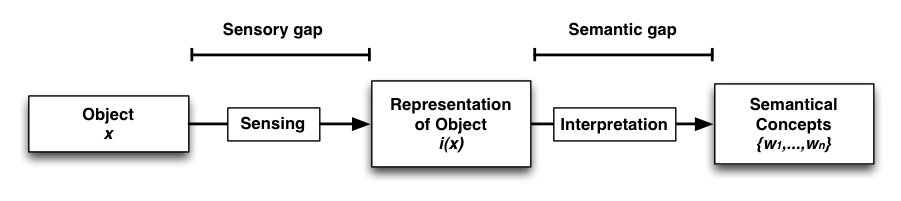
\includegraphics[width=.9\textwidth]{img/understanding_visuals}
  \caption{A high-level model of the interpretation of visual media content}
  \label{fig:understanding_visuals}
\end{figure}

% first problem: sensory gap
A first source of complication in the process from object to its interpretation, is the \emph{sensory gap}, described by Smeulders et al. as follows:

\begin{quote}
  ``The sensory gap is the gap between the object in the world and the information in a (computational) description derived from a recording of that scene.''\cite{Smeulders:2000tx}
\end{quote}

% sensory gap explained
The sensory gap makes accurate description of objects in the world difficult as it introduces uncertainty about what aspects of the object are represented. Characteristics of illumination, occlusion, clutter and camera viewpoint all affect the representation of a sensed object. When detailed knowledge about the recording conditions is absent, it is impossible to know which parts of the sensory information should be attributed to the state of the object and which are due to incidental artefacts. Different 3D objects can yield the same 2D representation and differently coloured objects might be represented by identical colour values. This also works the other way, as one object may appear very different in shape and colour on different images depending on illumination and camera viewpoint.

% second problem: semantic gap
A second and more challenging issue that hinders meaningful computational interpretation of visual content is the \emph{semantic gap} that lies between a digital representation and the conceptual interpretation we address to it. Snoek and Worring adapt the original definition from \cite{Smeulders:2000tx} to specifically fit the medium video when they describe the semantic gap as:

\begin{quote}
  ``The lack of correspondence between the low-level features that machines extract from video and the high-level conceptual interpretations a human gives to the data in a given situation.''\cite{Snoek:2009dq}
\end{quote}

The semantic gap makes automatic video categorisation and video concept detection difficult tasks\cite{Snoek:2009dq}. It also makes it hard for users searching in digital video systems to formulate their query in a way that matches the features accessible to the retrieval system.

One of the causes of the semantic gap is that the way people interpret images is mostly contextual\cite{Smeulders:2000tx}. We look for concepts that are already familiar from our environment or earlier encounters with visual content. Our perception of a simple object is determined by our vast background of personal experience and cultural upbringing. In contrast to these contextual interpretations, computational image descriptions rely purely on data-driven features that can be extracted from the content. Difficulties arise when there is a mismatch between the two.

% subjective interpretations; feeling and emotions
Another cause of the gap are interpretations that are subjective in nature. Semantical concepts relating to feelings and emotions can vary widely across different people. Deciding computationally whether concepts such as ``romantic'' or ``funny'' apply to a piece of content is hard when there is no agreement about the interpretation to begin with.

% concepts combined into larger meanings
Perceived concepts are also combined to infer a larger story around the things we actually see. These knowledge-based interpretations enable us to perceive deeper layers of meaning that are not in itself explicitly represented. An important example of this is the way `readers' of narrative texts or moving images combine elements in their aim for \emph{coherence}\cite[p.~38]{Bordwell:1985tz} \cite{gernsbacher1995coherence, Graesser:1994va}. High-level concepts like coherence over time are usually not explicitly represented in digital content and can be hard to compute algorithmically.

% large variety in appearance of visual concepts 
Even if there is little context dependency in the perception or recognition of an object in video, it might still be hard for computational methods to produce appropriate semantical labels. This is due to the wide variety in appearance of visual concepts. Determining whether a clock is present in a video can be difficult because of the many different sizes, shapes and colours clocks can have. 

All of these issues contribute to the gap between the low-level features extracted from video and the interpretations humans give to them. Challenges posed by the semantic gap are of mayor concern to the research community focussing on multimedia retrieval based on querying by user defined semantical concepts. The challenge is thus relevant to different scientific disciplines such as computer vision, information retrieval, machine learning and human-computer interaction. The next section briefly reviews computational strategies that aim to narrow the semantic gap.

% section challenges_in_computational_interpretation_of_visual_content (end)

\section{Computational Undertakings of the Quest for Meaning}

This section gives a short overview of strategies to narrow the semantic gap that is apparent in the computational interpretation of video content. At the core of this quest for meaning is the task of concept detection\cite{Snoek:2009dq}, where video clips are analysed to automatically detect whether a certain concept is present. Another step that is commonly taken to go from low-level video features to semantical interpretations is a classification of the type of content. This classification can be done at different levels, ranging from general and conceptually low-level (a scene containing music) to specific and conceptually high-level (a rock concert at an outdoor festival)\cite{Wang:2000vf}.

Before starting the processes of classification or concept detection, videos are usually segmented into smaller clips. The most common unit for temporal video segmentation is the \emph{shot}, one continuously recorded interval in the same setting of time and place. Shot segmentation is a well-understood problem and efficient automatic methods exist \cite{springerlink:10.1007/BF01210504, Yuan:hu}. Another form of partitioning is to segment the video into \emph{scenes}, possibly consisting of multiple shots, signifying a unit within a story\cite{Wang:2000vf}. While shot segmentation can be done automatically thanks to data-driven procedures, the task of scene segmentation relies on semantical and narrative interpretations of the content and is thus a lot harder to solve computationally.

The tasks of video classification and video concept detection, are generally organised as follows. For a video segment or keyframe $i$, represented by $n$-dimensional feature vector $x_i$, a measure is calculated that indicates whether conceptual label $\omega_j$ applies to shot $i$ (concept $w_j$ is present in $i$ or  $i$ can be classified as being of type $w_j$). The most common paradigm to find the relation between $x_i$ and $\omega_j$ is supervised learning. Supervised learning methods use a large number of examples in a training phase to find an optimal combination of features that codes for the presence of a particular concept. Using the found relationship from features to conceptual label, previously unseen instances can be classified with a certain accuracy. This section briefly addresses different features that can be extracted from video content and explains the general framework of supervised learning.

\subsection{Feature Extraction}

Video content has a multi-modal nature, and may consist of a recorded visual stream, animations, recorded or synthesised sounds, spoken language and textual information in (sub)titles, all presented in a sequential format over time. This rich nature of the medium makes that there are many different types of features that can be extracted from a piece of content. 

To help alleviate the semantic gap between low-level features and high-level interpretations, features should have enough discriminatory power to distinguish between the appearances of different concepts. Due to the sensory gap, variations in appearance also exist that are not caused by a difference in semantics, but are rather induced by the recording conditions. Features need so have a sufficient level of \emph{invariance} to these accidental visual distortions introduced by the sensory gap\cite{Smeulders:2000tx}. A higher level of invariance in the description of concept $w_j$ means the concept will be detected across a variety of different recording conditions. On the other hand the invariance might cause concept $w_j$ to be detected in the representation of other concepts with a similar appearance. Invariance thus comes at the cost of discriminatory power. In the choice of a feature set a balance should be sought between invariance and discrimination that is suitable for the particular domain of content and application. Most focus in feature extraction is on visual features, and we will start by indicating the types of features that are in use.

\subsubsection{Visual Features}
Despite the different modalities that can collectively make up a piece of video, it's defining characteristic is the presence of a sequence of images. Most efforts to narrow the semantic gap in video systems focus on the visual modality and try to make use of the features that can be extracted from it. In their wide-ranging overview of concept-based video retrieval techniques, Snoek and Worring point to the following types of visual features that are used in video concept detection\cite{Snoek:2009dq}.

\begin{itemize}
  \item \emph{Colour} - Colour can generally be represented in different 3D colour spaces (e.g. $rgb$, $hsv$ or $l*a*b$) and has discriminating potential superior to the single dimensional greyscale domain. In \cite{Smeulders:2000tx} Smeulders et al. indicate two aspects that have to be considered when working with colour features. First is the considerable variability in appearance of coloured surfaces under different recording circumstances, contributing to the sensory gap. Second is the intricacy of human colour perception that has to be accounted for in addressing visual interpretations approaching those brought forth in human experience.
  \item \emph{Texture} - While colour features can be calculated for every pixel in an image, texture features look at regions of multiple pixels to determine local patterns. Texture features are used to describe different materials or surfaces, for example the fine grained texture of sand versus the linear texture of hairs. A common practice is to capture directional patterns of texture using localised derivatives of changes in colour\cite{Jain:1991wc}. An example application of such methods is the detection of edges within an image.

  \item \emph{Shape} - When colours and textures of an image have been analysed, the resulting features can be used to partition images into smaller homogeneous areas. The shape of these areas can next be represented by features that either describe the shape's region or contour. Data-driven methods are used for \emph{weak segmentation}, where an image is deconstructed into shapes that share a visual property\cite{Veltkamp:2001vn}.  \emph{Strong segmentation} on the other hand, uses knowledge about the shapes of objects to delineate contours of semantic concepts in the image.

  \item \emph{Temporal} - Besides addressing aspects of single video frames, visual features can also capture how characteristics of frames develop over time. By following how sequential images change over time, patterns of motion can be tracked to describe camera motion\cite{Tonomura:1994vb}, motion of regions or points \cite{Sivic:2006jw} or even the movement of segmented objects\cite{Nguyen:2000vk}. A problem with using temporal features is that they are computationally costly and time-consuming to extract. This is a general problem with video induced by the sequential nature of consisting of information rich images. Because of this, temporal features are not commonly used in automated detection and categorisation methods.

\end{itemize}

\subsubsection{Auditory Features}

While video semantics might be most prominently expressed in the visual domain, auditory signals can also be used for segment-type classification and concept detection. In fact, auditory features may have the important advantage of being computationally cheaper relative to their visual counterparts. Considering this benefit, it can be strategic to start with an initial analysis of audio signals, and only proceed with more costly video analyses if further disambiguation is required. Different types of audio signals can be used for analyses 

As is the case for visual features, video content is first segmented before audio features are extracted. Generally, auditory feature extraction is done on two levels: short-term frame level and long-term clip level \cite{Wang:2000vf}. Frames are usually very short sample intervals spanning 10 to 40 ms, for which auditory signals are assumed to be stationary. Clips have longer durations that span multiple frames and are used to capture the changes in frame features over time.

In their overview of the merit of audio and visual features in the characterisation of semantic content, Wang et al. categorise audio features based on the type of information they are extracted from. They distinguish features based on \emph{volume}, \emph{zero crossing rate}, \emph{pitch} and \emph{spectral features}. Description of these features and their respective merit are left out of this thesis. Interested readers are referred to \cite{Wang:2000vf} for a detailed explanation. With frames analysed, features at clip level can be calculated to reflect the changes in frame level features over time. The different types of features on clip level can be characterised by the categories of the frame level features they are based on.

\subsubsection{Textual Features}

So far we've seen that auditory and visual information need interpretation to arrive at semantical concepts that can be expressed in text. In contrast to the sensory nature of audio and visuals, textual data is nice to deal with computationally as its symbolic nature makes it directly accessible to algorithmic processing. Not all videos feature text, but for certain types of video it is a viable option to extract textual information and use it for the characterisation of the video's semantics. Digital video files in itself do not contain textual data, but this can be extracted either from the visual or auditory stream.

Text might be available in a video's visual content in the form of titles or captions. It is mostly structured content, produced by a (semi-)professional editor that has these kinds of texts embedded. Video content following a fixed structure has the additional benefit of text elements appearing at regular times and positions. News programmes for example feature titles at fixed moments in time such as during the introduction of a person or location. \emph{Video optical character recognition} has been applied to news material to transcribe headline texts indicating topics of news items as well as to extract information about the text such as size and position\cite{Kuwano:2000wy}.

Another form of text from video is the transcription of spoken language in the audio stream. This is particularly interesting for video content that contains much information in spoken language, such as news programmes or other narrated presentations. For such content transcriptions may be present in the form of closed captions or extracted using \emph{automatic speech recognition}. Accurate transcriptions can lead to major improvements in interactive retrieval performance by novice users\cite{Christel:2005td}.

\subsection{Supervised Learning}

Once a suitable set of features is extracted for a collection of videos, they can be analysed to see how they relate to the concepts that are detected within the videos. The paradigm of supervised learning looks to find a relation between features describing data instances and classifications that can be attributed to them. Supervised learning takes place in two stages. In the initial training stage, a large set of training examples is taken along with the known classification or labels of the content.  Different methods can be used to determine a function that optimally describes how features are combined in the calculation of a measure that indicates whether the concept is present. During the testing stage the trained model is used with new instances as input (represented by the same set of features as the training examples) and calculates the probability $P(w_j | x_i)$ of concept $w_j$ being present in the video segment $i$ represented by feature vector $x_i$.

Although detectors can be trained to detect patterns of multiple concepts, usually separate concept detectors are trained for distinct concepts. By applying multiple detectors on an previously unseen input instance, multiple concepts can be detected.

\section{Outstanding Challenges} % (fold)
\label{sec:outstanding_challenges}

Despite significant advances have been made in recent years in methods to narrow the gap between low level video features and the high-level interpretations humans address to the content, the semantic gap still forms a major scientific challenge. The computational methods described in this chapter have clear values in addressing the semantic gap, but there are several difficulties that make it unlikely for the the gap to become bridged completely soon.

Although the low-level features described here can all be extracted automatically, the use of supervised learning methods still requires initial labelling from trusted sources. Acquiring these initial human labels might be costly and time-consuming.

Related to this is the idea that for accurate interpretations, a system might have to be updated to reflect newly added content or the latest contextual knowledge of its users. Periodical reassessment of feature sets or user-defined labels may prove impractical in an architecture based on supervised learning.

% temporal processing is computationally costly and time consuming
Processing visuals is a complex matter in its own right, but the temporal aspect of video adds an extra dimension of challenges. The sequential nature of video makes it a very information rich medium, with much to gain from but also much to be  challenged by. Looking at temporal features is costly and therefore currently left largely unexplored.

Even though the combination of low-level feature extraction and supervised learning builds a bridge across the semantic gap, these methods leave many intermediary levels of interpretation unaddressed. Of particular importance seem to be narrative analyses that characterise scenes within a video according to the role they play in a story. These features are very conceptual and thus hard to detect automatically by data-driven procedures based on low-level features. A second difficulty comes from the fact that characterisation of these concepts is hugely dependent on the context in which they are presented. Because narrative structure arises from sequential ordering of elements in time, it requires analysis that addresses a range of shots or scenes which is problematic because of aforementioned reasons. It has been shown that the configuration of elements in film and video can strongly affect the meaning that emerges from their assemblage. This property is dealt with extensively in studies of cinema\cite{Bordwell:1985tz} and is termed the `Kuleshov effect', after Lev Kuleshov who is an early investigator of this dependency effect:

\begin{quote}
  ``one must not forget that the location of the shot in a a montage phrase is crucial, because it is the position that, more often than not, explains the essence of the meaning intended by the artist-editor, his purpose (often the position in the montage alters the content).''\cite[``The Principles of Montage'']{kuleshov1974kuleshov}
\end{quote}

% wide domains e.g. ugvc
Perhaps the biggest challenge in the automatic interpretation of video is the wide variety of content that is produced and distributed nowadays. When considering ``\emph{narrow domains}'' of visual content, variations in appearance across different concepts are limited and predictable\cite{Smeulders:2000tx}. This makes narrow domains relatively easy to interpret as accidental distortions due to the sensory gap are limited. The contrary is true for broad domains:

\begin{quote}
  ``A broad domain has an unlimited and unpredictable variability in its appearance even for the same semantic meaning.''\cite{Smeulders:2000tx}
\end{quote}

The broader the domain, the wider the semantic gap. Phrased in the context of image retrieval, Smeulders et al. further illustrate the idea of broad domains by mentioning the set of images available on the internet as the broadest class available. The same can be said about video. Regarding the enormous amount of user-generated video content that are being uploaded, a platform like YouTube comes frighteningly close to this broadest scope. With so many users actively participating on such large scale platforms, extremely broad domains of video content become realities to be dealt with appropriately and this may prove a hurdle in the effort of solving the problems posed by the semantic gap.

% a way around the gap by asking people for their interpretations of content
Alternative to the approach of unleashing advanced number-crunching algorithms to try to achieve more meaningful interpretations computationally, there may be other ways that alleviate the problems posed by the semantic gap. The next chapter looks at methodologies that have at their core the idea of accessing people's interpretations to support digital systems in tasks that are currently hard to solve computationally. Considering the outstanding challenges due to the semantic gap in automatic video interpretation, these methods may prove especially rewarding for the medium of digital video.

% section outstanding_challenges (end)



% \subsection{Structural Features}
% 
% [cite bordwell \& Thompson: analysis of context dependency]
% 
% 
% % hypervideo as form of 1 narrative 2 navigation, link to database documentary
% [HyperCafe: Narrative and Aesthetic Properties of Hypervideo \cite{Sawhney:1996tk}]
% 
% 
% \section{Interactive Storytelling: From database to data-based}
% 
% \subsection{Symbolic approaches to storytelling}
% \cite{Vilmos:2011wv,RodrigoLaiolaGuimaraes:2011tl,Ursu:2009gc}
% 
% \subsection{Statistic, emergent approaches}
% \label{sec:statistic}
% 
% NLP
% 
% \subsection{Remixing}
% 
% The reconfiguration of smaller units that carry meaning within themselves is common practice for textual media such as blogs, where it is easy to quote part of  another author`s writing in a new post [ref]. 
% 
% It needs to be said that some reconfiguration of videos is taking place, but even though it often concerns content that was originally sourced online, much of the creative act of remixing happens offline.
% 
% 
% % Taking the remix online
% 
% examples like: Aaron Koblin (johnny cash project, exquisite corps, etc)
% 
% there is even word of a true remix culture\cite{Diakopoulos:2007tl}.
% 
% the availability of multimedia content via the internet has meant a surge in 
% 
% \section{Discussion} % (fold)
% \label{sec:discussion}
% 
% 
% \subsection
% Human interaction [Relevance feedback: A power tool for interactive content-based image retrieval]\cite{Rui:1998uj}
% [collaborative filtering] \url{http://en.wikipedia.org/wiki/Collaborative_filtering}
% 
% 
% % section discussion (end)
% 
% 
% 
% 
